\documentclass[journal]{IEEEtran}
\usepackage{cite}
\usepackage{graphicx}
\usepackage{booktabs}
\usepackage{amsmath}
\usepackage{amssymb}
\usepackage{placeins}
\usepackage{array}
\usepackage[hidelinks]{hyperref}
% Generated from results/*.json; do not edit by hand.
\newcommand{\DataRows}{283726}
\newcommand{\FraudCount}{473}
\newcommand{\BestModel}{pending}
\newcommand{\BestPRAUC}{pending}

\title{Leakage-Aware Credit-Card Fraud Detection Under Temporal Evaluation}
\author{S.~Yaswanth~Krishna~Chaitanya\\
\textit{Indian Institute of Information Technology Nagpur}\\
\texttt{bt25csd028@iiitn.ac.in}}
\begin{document}
\maketitle

\begin{abstract}
Credit-card fraud detection is a rare-event problem in which random partitions, full-data preprocessing, and test-selected thresholds can make reported performance optimistic. We evaluate the ULB credit-card dataset after exact duplicate removal using contiguous chronological training, validation, and holdout partitions; fold-local preprocessing and imbalance handling; stratified cross-validation; validation-selected operating thresholds; and bootstrap uncertainty intervals. The comparison includes \ModelFamilyCount{} model families and the available class-weighting, synthetic oversampling, and undersampling strategies. Cross-validation selected XGBoost with class weights as the primary candidate, with mean average precision (AP) \PrimaryCVAP{} (fold standard deviation \CVBestSD{}). Its single holdout AP was \PrimaryHoldoutAP{} (stratified-bootstrap \ConfidenceLevel{}\% CI [\PrimaryHoldoutAPLow{}, \PrimaryHoldoutAPHigh{}]). An all-legitimate classifier achieved accuracy \AllLegitAccuracy{} while the dummy AP was \DummyAP{}. The paired interval for the two leading candidates by cross-validation includes zero, so their holdout rankings are not clearly separated. Development-only protocol ablations show larger changes for XGBoost than for the forest, but bundle multiple changes and do not identify a causal leakage effect. The study spans only \TimeSpanHours{} elapsed hours and cannot establish deployment performance or long-term drift robustness.
\end{abstract}

\begin{IEEEkeywords}
Credit-card fraud detection, class imbalance, temporal evaluation, data leakage, average precision, model calibration.
\end{IEEEkeywords}

\section{Introduction}
\label{sec:introduction}
Credit-card fraud detection is difficult for two related reasons: fraudulent transactions are rare, and transaction patterns can change over time. In this dataset, an all-legitimate decision rule attains accuracy \AllLegitAccuracy{} while the dummy class-prior model has AP \DummyAP{} (Table~\ref{tab:holdout-ranking}); the apparent accuracy therefore says little about how well fraud is ranked. Average precision (AP, equal to PR-AUC here) emphasizes performance on the positive class and is the primary ranking measure in this study \cite{saito2015}.

Evaluation design can make a fraud model appear stronger than it is. If a scaler, resampler, threshold, or candidate model is selected using information from an evaluation partition, the estimate no longer represents a clean learn-then-predict process \cite{kaufman2012}. Broader concerns about leakage and reproducibility in machine-learning studies motivate an explicit record of the choices made from development data and the final holdout \cite{kapoor2022}. Operational fraud systems also face delayed verification and changing transaction behavior; a short chronological evaluation is relevant to those concerns but cannot demonstrate resistance to long-term drift \cite{dalpozzo2018}.

This paper makes four contributions:
\begin{enumerate}
  \item It evaluates five non-dummy model families with fold-local preprocessing and imbalance strategies under train-only cross-validation, followed by validation-based thresholds and a single chronological holdout evaluation.
  \item It reports candidate metrics symmetrically with stratified-bootstrap intervals and paired post-hoc AP differences, distinguishing the candidate selected by cross-validation from the candidate with the largest observed holdout AP.
  \item It measures protocol-specific development results, model attribution, error profiles, calibration, and an illustrative review-cost sensitivity analysis without interpreting anonymized components as business causes.
  \item It documents the remaining limits of the evidence, including the short time span, small fraud counts in validation and holdout, and the non-causal nature of the bundled ablation.
\end{enumerate}
The remainder of the paper describes the data and models, specifies the evaluation procedure, reports the results, and discusses limitations and deployment needs.
\FloatBarrier

\section{Related Work}
\label{sec:related}
Prior work associated with the ULB credit-card dataset addresses probability calibration under undersampling and the practical conditions of fraud detection, including delayed labels and non-stationarity \cite{dalpozzo2015,dalpozzo2018}. Those studies motivate the use of time-aware partitions and attention to probability behavior; they do not establish the results of the present experiments or show that this short split solves drift.

Class weighting changes the loss assigned to errors, while random undersampling changes the training class composition. Prior work reports posterior-probability effects of undersampling \cite{dalpozzo2015}. SMOTE interpolates minority-class examples, but its original experiments do not establish improved boosting performance or improved AP for this dataset \cite{chawla2002}. The strategies are therefore compared empirically, with resampling confined to the training portion of each fold.

For strongly imbalanced evaluation, precision-recall analysis makes the positive-class trade-off visible, while the Matthews correlation coefficient (MCC) provides a measure that uses all four confusion-matrix cells \cite{saito2015,chicco2020}. The study reports accuracy only as context, alongside AP, ROC-AUC, threshold metrics, MCC, and a fixed alert-budget measure.

Leakage research formalizes the separation between information available during learning and information available at prediction time \cite{kaufman2012}. Work on leakage and reproducibility further argues for documenting the full evaluation process \cite{kapoor2022}. This paper adds a comparison of candidate pipelines under a chronological holdout, a development-only protocol ablation, and an explicit report of which conclusions are supported by overlapping or non-overlapping uncertainty intervals.
\FloatBarrier

\section{Dataset and Exploratory Analysis}
\label{sec:data}
The ULB transaction data contains anonymized principal-component features \texttt{V1}--\texttt{V28}, a transaction amount, elapsed time, and a binary fraud label. The time variable is seconds since the first transaction, not wall-clock time. After exact duplicate removal, the analysis contains \DataRows{} transactions and \FraudCount{} fraud cases from \RawRows{} raw rows; the elapsed span is \TimeSpanHours{} hours (Table~\ref{tab:splits}). No card or merchant identifiers are available, so the anonymized components cannot be translated into customer, merchant, or transaction mechanisms.

Table~\ref{tab:splits} gives the contiguous time ranges and class rates. The validation fraud rate is about half the training rate (\ValidationFraudRateRatio{} of it), which indicates that class prevalence changes across these adjacent periods. Fig.~\ref{fig:data-overview} combines the class distribution and within-train hourly patterns: the imbalance makes AP and alert precision/recall more informative than accuracy, while time variation supports preserving order and deriving cyclical time features. These descriptive patterns do not by themselves establish a deployment drift process.

\begin{table}[!t]
\centering
\caption{Chronological data partitions after exact duplicate removal. Time is elapsed from the first transaction.}
\label{tab:splits}
\begin{tabular}{lrrrr}
\toprule
Split & Rows & Frauds & Fraud rate & Time (h) \\
\midrule
Train & 170,235 & 342 & 0.201\% & 0.000--33.442 \\
Validation & 56,745 & 57 & 0.100\% & 33.443--40.343 \\
Test & 56,746 & 74 & 0.130\% & 40.343--47.998 \\
\bottomrule
\end{tabular}

\end{table}

Amount distributions overlap across classes, so amount alone is not a sufficient separator. The train-only marginal screens also rank components differently by effect size and mutual information; Fig.~\ref{fig:eda} therefore motivates combining amount with the anonymized components and treating univariate rankings as descriptive rather than as model importance.
\begin{figure*}[!t]
\centering
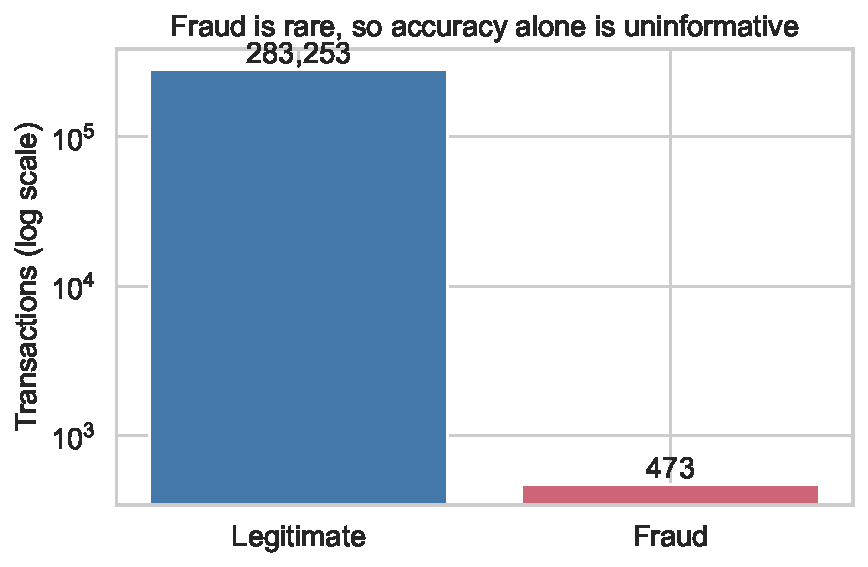
\includegraphics[width=0.48\textwidth]{figures/f01_class_imbalance.pdf}\hfill
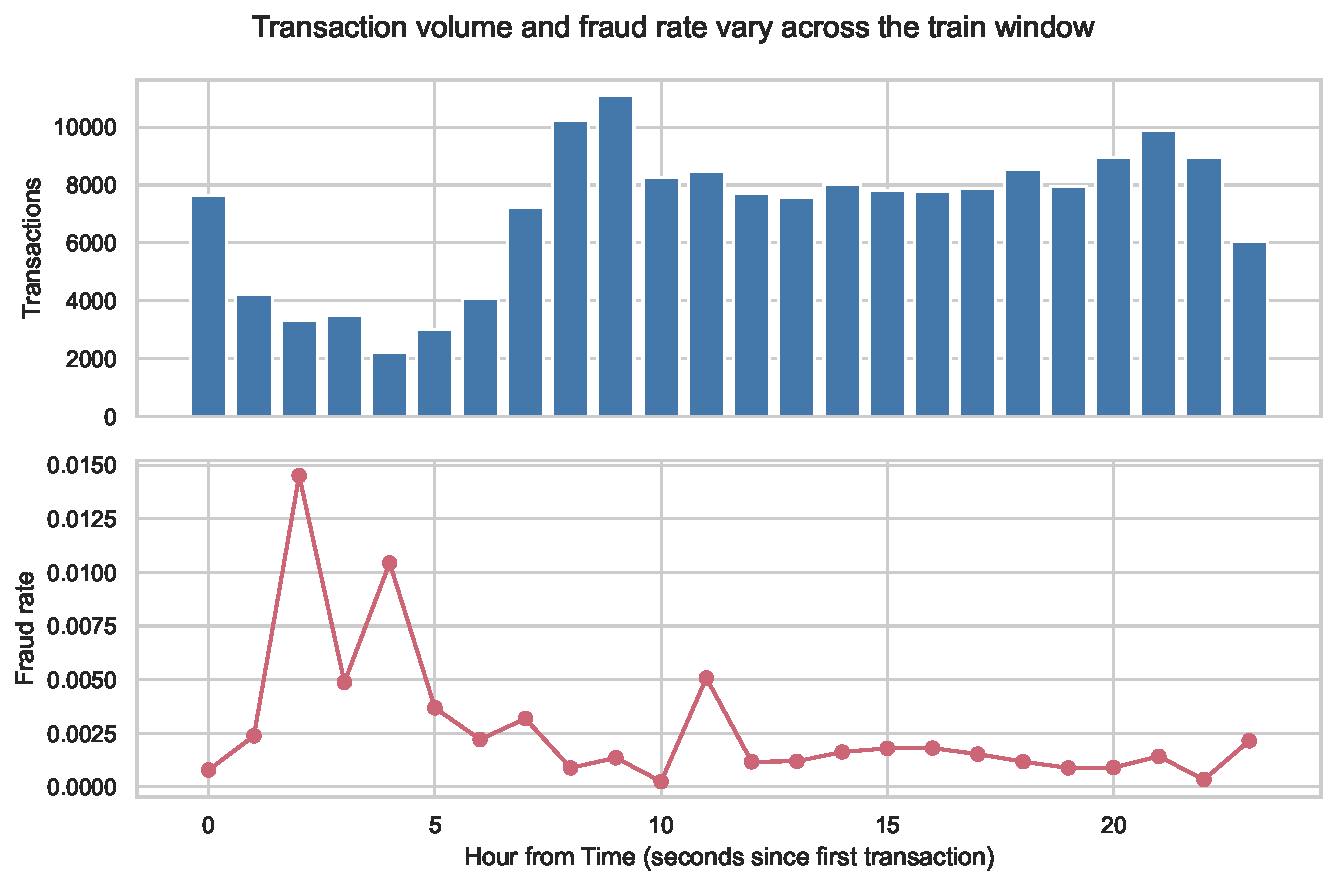
\includegraphics[width=0.48\textwidth]{figures/f02_hourly_patterns.pdf}
\caption{Dataset overview. (a) The fraud class is rare in the deduplicated dataset, so accuracy alone can be misleading. (b) Transaction volume and fraud rate vary by elapsed hour within the training interval, supporting chronological evaluation and cyclical time features.}
\label{fig:data-overview}
\end{figure*}

Fig.~\ref{fig:eda} pairs the amount ECDF with the train-only screens. The broad overlap in amounts argues against amount-only decisions, while disagreements among marginal screens call for multivariate validation rather than causal or business interpretations.
\begin{figure*}[!t]
\centering
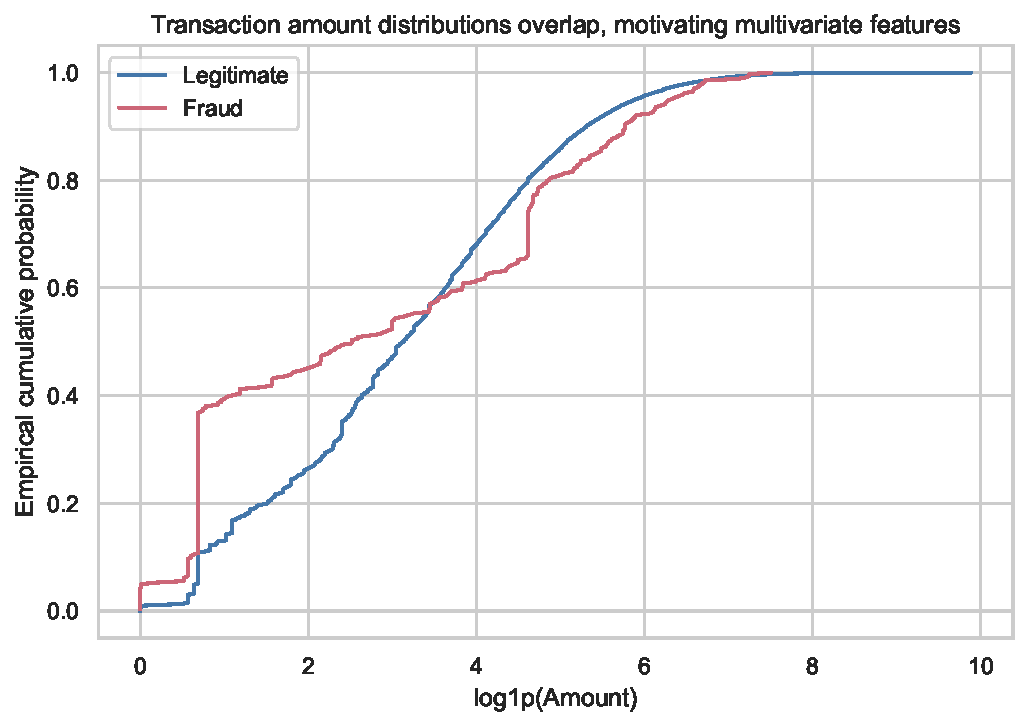
\includegraphics[width=0.48\textwidth]{figures/f03_amount_ecdf.pdf}\hfill
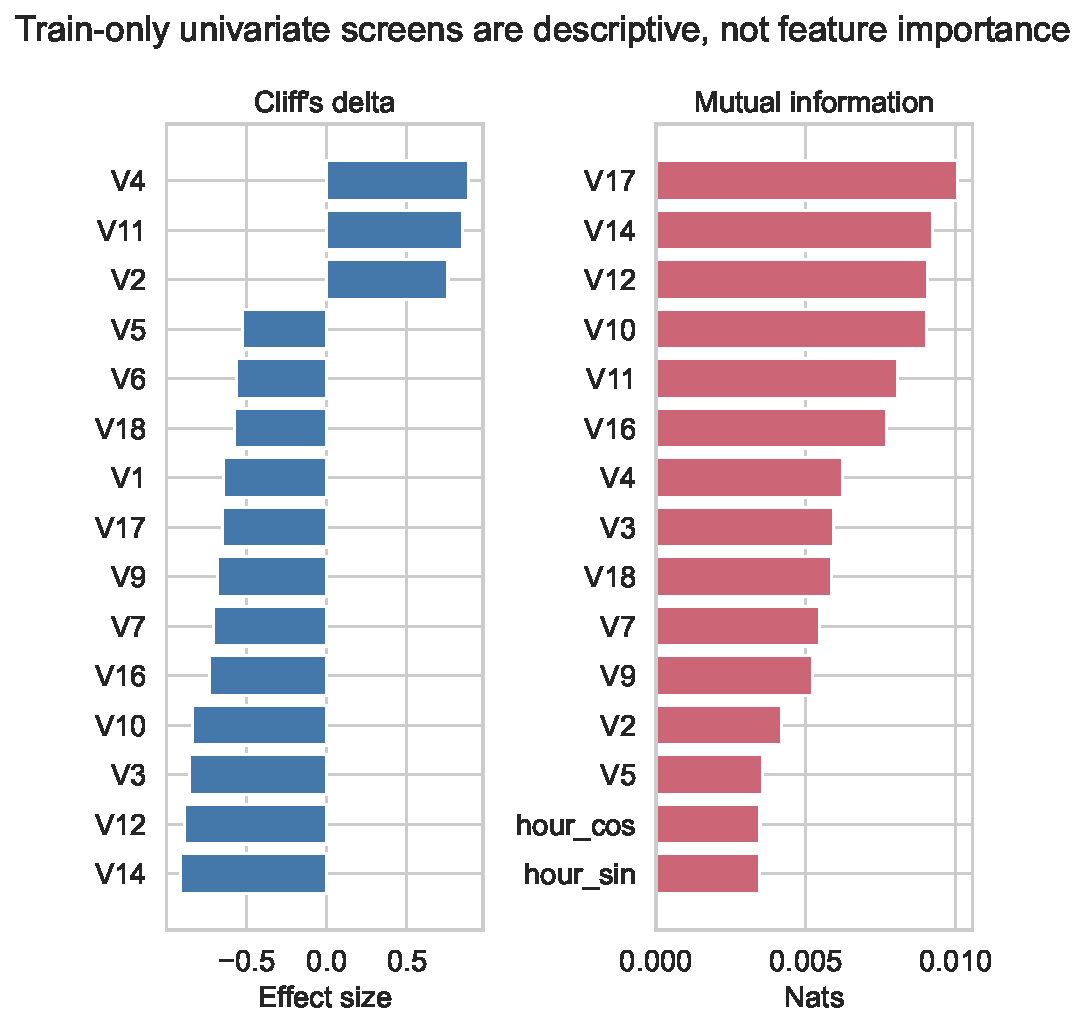
\includegraphics[width=0.48\textwidth]{figures/f04_feature_screens.pdf}
\caption{Exploratory findings. (a) Log-amount empirical distributions overlap between classes. (b) Effect-size and mutual-information rankings differ; they are descriptive screens and are checked against model-based attribution later.}
\label{fig:eda}
\end{figure*}
\FloatBarrier

\section{Models and Imbalance Strategies}
\label{sec:models}
Table~\ref{tab:model-rationale} summarizes the mechanism, reason for inclusion, and principal limitation of each model family. The selected settings are listed separately in Appendix~\ref{app:settings}; strategy-specific comparisons appear in Table~\ref{tab:cv}.

\begin{table*}[!t]
\centering
\caption{Model families, rationale, and limitations for this numeric, anonymized dataset.}
\label{tab:model-rationale}
\begin{tabular}{p{0.12\textwidth}p{0.24\textwidth}p{0.27\textwidth}p{0.25\textwidth}}
\toprule
Model & Mechanism & Advantage & Limitation in this study \\
\midrule
Class-prior dummy & Predicts the training class prior & Defines a no-skill ranking reference & Does not learn transaction structure \\
Logistic regression & Linear decision boundary with regularized coefficients & Convex, fast, and readable; useful for linear PCA projections & May miss interactions and is sensitive to scale and heavy-tailed amount \\
Random forest & Bagged decision trees & Captures nonlinearities and interactions without feature scaling \cite{breiman2001} & Vote-based probabilities can be coarse and cannot extrapolate beyond observed feature ranges \\
K-nearest neighbors & Distance-weighted local voting with $k$ set in the saved configuration & Simple nonparametric reference for local structure & Distance is difficult in high dimensions; minority neighbors are sparse and prediction is expensive \\
XGBoost & Regularized gradient-boosted trees with histogram splits & Shrinkage, subsampling, and class weighting provide a strong CPU-capable comparator \cite{chen2016} & Several interacting settings and few positive cases can make overfitting and probability calibration concerns \\
CatBoost & Symmetric trees with ordered boosting & Ordered boosting targets prediction shift \cite{prokhorenkova2018} & Slower on CPU; categorical-feature machinery is irrelevant because these features are numeric \\
\bottomrule
\end{tabular}
\end{table*}

Logistic regression tests whether a linear boundary on the PCA-derived variables is competitive. Its class-weighted and SMOTE CV AP values are \LRWeightsCVAP{} and \LRSmoteCVAP{} (Table~\ref{tab:cv}); neither reaches the leading tree candidates. The hypothesis of competitive ROC-AUC but weaker AP is only partly resolved: the saved hypothesis log marks the ROC-AUC comparison inconclusive and the AP comparison weaker.

The forest tests nonlinear interactions with comparatively coarse vote probabilities. The class-weighted forest was not one of the three locked holdout candidates, so its proposed moderate-recall operating behavior was not tested on the holdout; the selected forest configuration uses SMOTE. The holdout results for that selected configuration are reported alongside the other candidates rather than used to revise the selection.

K-nearest neighbors uses distance weights and the configured neighborhood size. It does not use resampling or undersampling, since SMOTE would make CPU prediction costly. The hypothesis that it would be the weakest model is refuted: its no-resampling CV AP exceeds the logistic-regression settings and the undersampling variants, although it remains below the strongest tree configurations (Table~\ref{tab:cv}).

XGBoost with class weights has the largest mean CV AP among the tested pairs and is declared the primary candidate before the holdout results are considered. CatBoost with class weights is close in CV mean and fold variability; the paired top-two interval does not establish a holdout difference. CatBoost's ordered boosting is relevant to prediction shift; its categorical-feature machinery provides no advantage here because the inputs are numeric.

The study compares class weights, SMOTE, and random undersampling. Weighting changes error costs without adding synthetic examples; SMOTE interpolates minority neighbors and may create unrealistic points in PCA space; undersampling is inexpensive but discards majority examples and can alter posterior probabilities \cite{dalpozzo2015,chawla2002}. On average across the available CV pairs, the saved strategy means are \WeightsStrategyMeanAP{} for weights, \SmoteStrategyMeanAP{} for SMOTE, and \UndersampleStrategyMeanAP{} for undersampling (Table~\ref{tab:cv}). These aggregate values are descriptive because the strategy groups contain different model families; per-model comparisons are given in the table.
\FloatBarrier

\section{Methodology}
\label{sec:method}
\subsection{A. Data preparation and chronological partitions}
Exact duplicates are removed, rows are stably sorted by elapsed time, and contiguous train, validation, and test partitions are created using the saved split proportions. Their row counts, fraud rates, and elapsed ranges are reported in Table~\ref{tab:splits}. The holdout is the latest partition; the earlier portions are used for training, model comparison, and threshold selection.

\subsection{B. Feature construction}
The model input contains the anonymized components, $\log(1+\mathrm{Amount})$, and cyclical encodings of the elapsed hour. Raw time is excluded because its absolute value is not a wall-clock timestamp and would invite direct use of the observed sequence index. The cyclical representation gives nearby hours similar encodings while retaining within-day patterns. No fitted statistic is used to construct these derived features.

\subsection{C. Leakage control}
Fig.~\ref{fig:protocol} shows the order of information use. Every resampling operation and scaler is fit only on the training part of a fold, validation labels select thresholds, and the final chronological partition is kept for the locked evaluation.
\begin{enumerate}
  \item For each cross-validation fold, fit the model pipeline, including any scaler and resampler, on that fold's training rows only.
  \item Score the held-out fold to estimate AP and secondary ranking metrics; aggregate the saved fold results for selection.
  \item Fit each locked candidate using the training partition and choose its operating thresholds using validation predictions and labels.
  \item Evaluate the locked candidates on the chronological test partition once and compute the specified bootstrap intervals.
  \item After that evaluation, compute the requested all-pairs AP intervals from the saved test predictions as a post-hoc descriptive analysis; do not use these intervals to make choices.
\end{enumerate}
\begin{figure*}[!t]
\centering
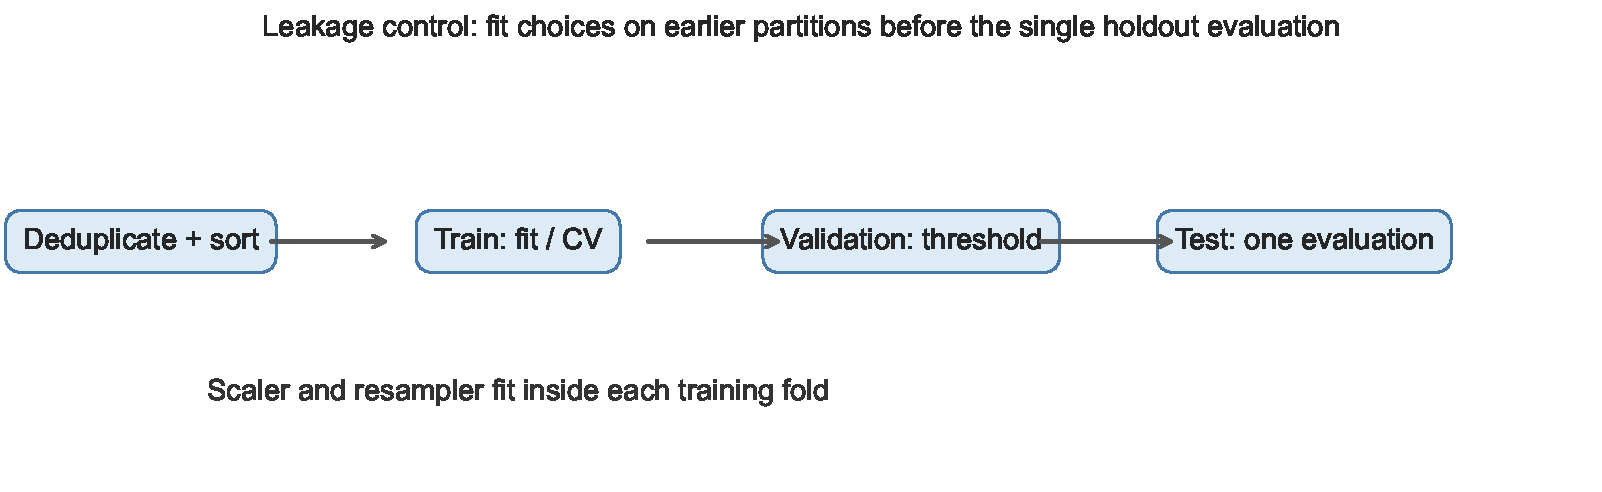
\includegraphics[width=0.95\textwidth]{figures/f06_leakage_protocol.pdf}
\caption{Evaluation sequence. Fitted preprocessing and resampling remain inside training folds, validation is used for threshold selection, and the chronological holdout is evaluated after choices are locked.}
\label{fig:protocol}
\end{figure*}

\subsection{D. Model and strategy selection}
Model and strategy selection uses stratified \CVFoldCount-fold cross-validation on the training partition, with AP as the primary score. The one-standard-error rule identifies candidates within the best mean minus one standard error; among that set, the measured fit time favors the faster candidate. The selected primary pair is \PrimaryModel{} at mean CV AP \PrimaryCVAP{} (Table~\ref{tab:cv}). The three locked holdout candidates all fall within the one-standard-error band (\CVTopThreeWithinOneSE{}; cutoff \CVOneSECutoff{}).

\subsection{E. Threshold selection}
For each locked candidate, the F1-maximizing threshold is chosen on validation data. A second operating point seeks the greatest recall among thresholds satisfying the high-precision constraint in the saved evaluator. Threshold values are model-specific and are not comparable as common risk cutoffs: weighting and SMOTE can alter probability scales, and validation contains only \ValidationFraudCount{} fraud examples (Table~\ref{tab:holdout-thresholds}).

\subsection{F. Metrics}
For binary predictions, precision, recall, F1, and MCC are defined as
\begin{align}
\mathrm{Precision} &= \frac{TP}{TP+FP},\\
\mathrm{Recall} &= \frac{TP}{TP+FN},\\
F_1 &= \frac{2\,\mathrm{Precision}\,\mathrm{Recall}}{\mathrm{Precision}+\mathrm{Recall}},\\
\mathrm{MCC} &= \frac{TP\,TN-FP\,FN}{\sqrt{(TP+FP)(TP+FN)(TN+FP)(TN+FN)}}.
\end{align}
AP summarizes precision over recall as the score threshold varies. It is the primary measure because class prevalence is low and accuracy can be dominated by legitimate transactions \cite{saito2015}. ROC-AUC, MCC, threshold precision/recall/F1, and precision at the fixed alert budget provide complementary views; MCC is not assumed to be stable under extreme imbalance \cite{chicco2020}.

\subsection{G. Uncertainty and post-hoc pairwise analysis}
The saved test intervals use stratified bootstrap resampling of positive and negative cases. The post-hoc pairwise comparison reuses the saved test labels and probabilities, draws \BootstrapReplicates{} paired stratified samples with the configured seed, and estimates AP differences for all pairs of locked candidates. The differences and intervals are descriptive only; no model, threshold, or hyperparameter choice depends on them. An interval containing zero is described as no evidence of a difference.

\subsection{H. Protocol ablation}
The ablation uses development data only. A0 is a legacy-like random evaluation with full-development scaling, SMOTE, and threshold selection on that evaluation partition; A1 moves scaling into the training pipeline; A2 selects the threshold on a random validation partition; A3 uses contiguous chronological development partitions. Each contrast changes multiple elements across stages, so the A0-to-A3 difference cannot be attributed to scaling leakage alone. The primary holdout does not enter this ablation.
\FloatBarrier

\section{Experimental Setup}
\label{sec:setup}
All model fitting used CPU implementations configured for an Intel i7-class processor with no GPU. The random seed in the saved configuration is \SeedValue{}; the full-run settings and average per-fold fit times for each model-strategy pair are listed in Appendix~\ref{app:settings} and Table~\ref{tab:cv}. The five-fold CV grid contains \CVPairCount{} model-strategy pairs; their total recorded fit time is about \CVTotalFitMinutes{} minutes, excluding data preparation and report-generation overhead. The FAST smoke run was not used to select models. Software versions below describe the environment used to regenerate the report assets; exact package versions for each original training process were not separately recorded.

\begin{table}[!t]
\centering
\caption{Software versions in the report-build environment.}
\label{tab:software}
\begin{tabular}{lr}
\toprule
Component & Version in report-build environment \\
\midrule
Python & 3.11.9 \\
platform & Windows-10-10.0.26200-SP0 \\
NumPy & 2.4.6 \\
pandas & 3.1.0 \\
SciPy & 1.17.1 \\
scikit-learn & 1.9.1 \\
imbalanced-learn & 0.14.2 \\
XGBoost & 3.2.0 \\
CatBoost & 1.2.10 \\
Matplotlib & 3.11.2 \\
SHAP & 0.51.0 \\
\bottomrule
\end{tabular}

\end{table}

\noindent\textbf{Reproducibility:} The report tables, macros, and package can be regenerated from the saved analysis outputs with \texttt{python scripts/export\_report\_assets.py}; this step does not fit a model.
\FloatBarrier

\section{Results}
\label{sec:results}
\subsection{A. Cross-validation model and strategy comparison}
XGBoost with class weights is the highest-mean CV pair at AP \XgbWeightsCVAP{} (fold SD \XgbWeightsCVSD{}). The next two locked candidates are CatBoost with class weights at \CatboostWeightsCVAP{} (SD \CatboostWeightsCVSD{}) and the forest with SMOTE at \RfSmoteCVAP{} (SD \RfSmoteCVSD{}); all three lie within one standard error of the leading mean. Table~\ref{tab:cv} presents all evaluated model-strategy rows and fit times, and Fig.~\ref{fig:cv} displays their fold means and variability. The standard deviations are about \CVBestSD{}, so the small mean differences among the leading candidates should not be treated as a stable ranking.

Undersampling has lower mean AP than both class weights and SMOTE for each tree model, and it is lower than SMOTE and weights for logistic regression; for logistic regression, SMOTE's mean is slightly above weights. KNN with no resampling exceeds the logistic-regression settings but remains below the strongest tree pairs (Table~\ref{tab:cv}). These comparisons support the reported strategy-specific findings without implying that a single imbalance strategy is uniformly best for every model.

\begin{table*}[!t]
\centering
\caption{Five-fold stratified training-CV average precision and mean fit time per fold. Entries are mean $\pm$ standard deviation across folds.}
\label{tab:cv}
\begin{tabular}{lrrr}
\toprule
Model & Strategy & AP (mean $\pm$ SD) & Fit (s) \\
\midrule
catboost & smote & $0.856 \pm 0.049$ & 20.071 \\
catboost & undersample & $0.660 \pm 0.075$ & 2.631 \\
catboost & weights & $0.868 \pm 0.050$ & 12.219 \\
knn & none & $0.824 \pm 0.039$ & 0.131 \\
knn & undersample & $0.707 \pm 0.074$ & 0.162 \\
lr & smote & $0.720 \pm 0.061$ & 0.964 \\
lr & undersample & $0.617 \pm 0.074$ & 0.105 \\
lr & weights & $0.711 \pm 0.072$ & 0.288 \\
rf & smote & $0.867 \pm 0.050$ & 104.178 \\
rf & undersample & $0.719 \pm 0.055$ & 0.583 \\
rf & weights & $0.858 \pm 0.048$ & 32.652 \\
xgb & smote & $0.861 \pm 0.055$ & 8.491 \\
xgb & undersample & $0.735 \pm 0.084$ & 0.303 \\
xgb & weights & $0.872 \pm 0.052$ & 4.973 \\
\bottomrule
\end{tabular}

\end{table*}

Fig.~\ref{fig:cv} shows the fold mean and standard deviation for every evaluated pair. The leading means are close relative to fold variability, while undersampling is consistently lower for the tree families; together, the table and plot favor reporting the candidates as close rather than claiming a decisive winner.
\begin{figure*}[!t]
\centering
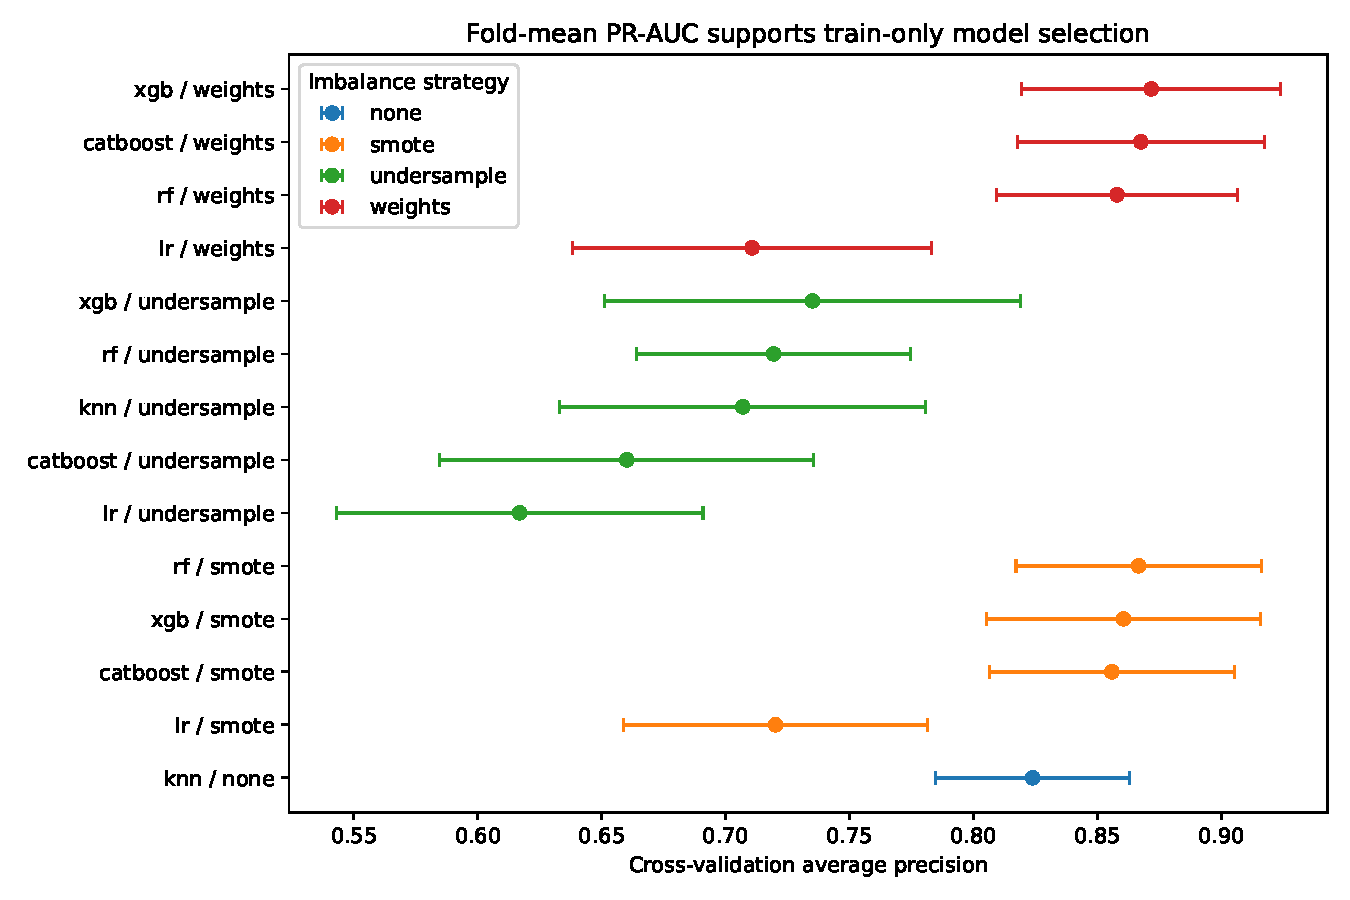
\includegraphics[width=0.95\textwidth]{figures/f07_cv_pr_auc.pdf}
\caption{Training-only cross-validation AP by model and imbalance strategy; points show fold means and horizontal bars show fold standard deviations.}
\label{fig:cv}
\end{figure*}

\subsection{B. Locked chronological holdout}
The CV-selected primary candidate is XGBoost with class weights, declared before the holdout evaluation; its holdout AP is \XgbWeightsAP{} with a stratified-bootstrap interval shown in Table~\ref{tab:holdout-ranking}. The forest with SMOTE has the numerically largest holdout AP, \RfSmoteAP{}, while CatBoost with class weights has AP \CatboostWeightsAP{}. Table~\ref{tab:holdout-ranking} reports AP and ROC-AUC with intervals for all three; Table~\ref{tab:holdout-thresholds} reports their validation-selected operating points. Fig.~\ref{fig:holdout} pairs the PR curves with confusion matrices, whose axes use actual class by row and predicted class by column.

The dummy AP is \DummyAP{}, while the all-legitimate accuracy is \AllLegitAccuracy{}; the latter is not a fraud-detection success measure. The XGBoost and forest thresholds yield identical TP, FP, and FN counts in Table~\ref{tab:holdout-thresholds}, despite different score rankings. The post-hoc XGBoost-minus-CatBoost paired AP difference is \TopCVPairDifference{} (\ConfidenceLevel{}\% CI [\TopCVPairLow{}, \TopCVPairHigh{}]), which includes zero. The XGBoost-minus-forest interval is [\XGBRFPairLow{}, \XGBRFPairHigh{}], also including zero, whereas the CatBoost-minus-forest interval is [\CatRFPairLow{}, \CatRFPairHigh{}]. The latter is post-hoc and is not used to revise the CV-based choice.

The CV-to-holdout AP gaps are \XgbWeightsCVToHoldoutAPDrop{} for XGBoost, \CatboostWeightsCVToHoldoutAPDrop{} for CatBoost, and \RfSmoteCVToHoldoutAPDrop{} for the forest. A change in fraud prevalence across time and the limited holdout fraud count (\TestFraudCount{}) are plausible contributors, but this experiment does not identify their individual effects.

\begin{table*}[!t]
\centering
\caption{Locked chronological holdout ranking metrics with stratified-bootstrap \ConfidenceLevel{}\% confidence intervals.}
\label{tab:holdout-ranking}
\begin{tabular}{lrr}
\toprule
Model/strategy & AP [95\% CI] & ROC-AUC [95\% CI] \\
\midrule
xgb/weights & 0.795 [0.706, 0.876] & 0.973 [0.949, 0.990] \\
catboost/weights & 0.784 [0.698, 0.865] & 0.957 [0.921, 0.986] \\
rf/smote & 0.812 [0.728, 0.890] & 0.969 [0.946, 0.989] \\
\bottomrule
\end{tabular}

\end{table*}

\begin{table*}[!t]
\centering
\caption{Holdout threshold metrics at thresholds selected on validation data; counts are true positives, false positives, and false negatives.}
\label{tab:holdout-thresholds}
\begin{tabular}{lrrrrrrrr}
\toprule
Model/strategy & Threshold & Prec. & Recall & F1 & MCC & TP & FP & FN \\
\midrule
xgb/weights & 0.913 & 0.902 & 0.743 & 0.815 & 0.818 & 55 & 6 & 19 \\
catboost/weights & 0.970 & 0.864 & 0.689 & 0.767 & 0.772 & 51 & 8 & 23 \\
rf/smote & 0.539 & 0.902 & 0.743 & 0.815 & 0.818 & 55 & 6 & 19 \\
\bottomrule
\end{tabular}

\end{table*}

Fig.~\ref{fig:holdout} shows that AP ranking and a single threshold's confusion counts answer different questions. The overlapping paired intervals for the CV top pair and for XGBoost versus the forest mean there is no evidence of a difference for those pairs under this holdout sample.
\begin{figure*}[!t]
\centering
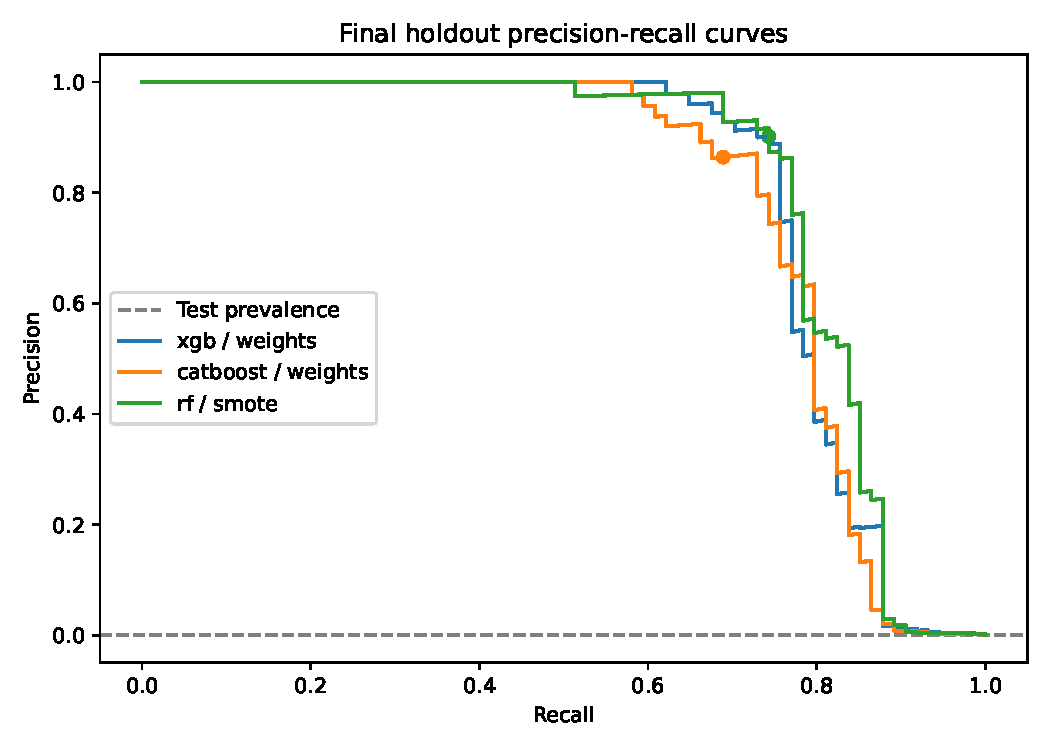
\includegraphics[width=0.48\textwidth]{figures/f08_test_pr_curves.pdf}\hfill
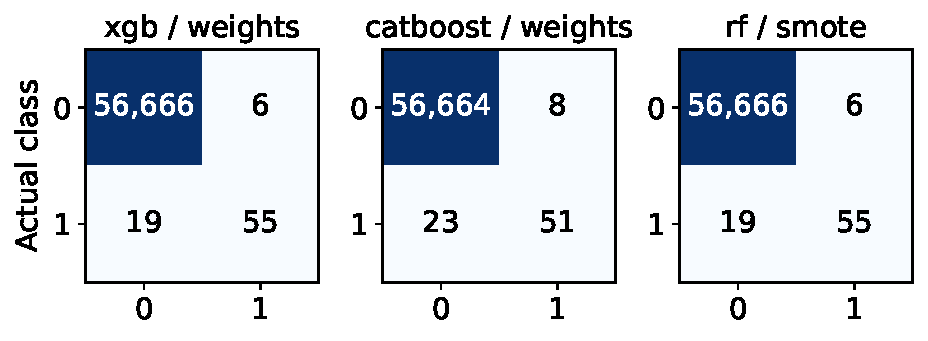
\includegraphics[width=0.48\textwidth]{figures/f09_confusion_matrices.pdf}
\caption{Locked holdout comparison. (a) Precision-recall curves and validation-selected F1 operating points show ranking behavior over thresholds. (b) Confusion matrices show actual class in rows and predicted class in columns; XGBoost and the forest have identical TP/FP/FN counts.}
\label{fig:holdout}
\end{figure*}

\subsection{C. Threshold behavior}
The F1-optimal validation thresholds are \XgbWeightsThreshold{} for XGBoost, \CatboostWeightsThreshold{} for CatBoost, and \RfSmoteThreshold{} for the forest (Table~\ref{tab:holdout-thresholds}). These values are not common risk cutoffs: model probability scales differ, particularly across weighting and SMOTE. The validation set has \ValidationFraudCount{} frauds, so its threshold estimates can be sensitive to a small number of cases. At the precision-constrained validation operating point, XGBoost's threshold is \XgbWeightsStrictThreshold{} and its holdout recall is \XgbWeightsRecallAtStrictThreshold{}; this is a separate operating point from the F1 threshold.

Fig.~\ref{fig:thresholds} plots validation F1 over threshold and marks the selected operating regions. The curves show why threshold values should be interpreted within each model's score scale rather than compared as though the numerical thresholds were calibrated to the same risk.
\begin{figure*}[!t]
\centering
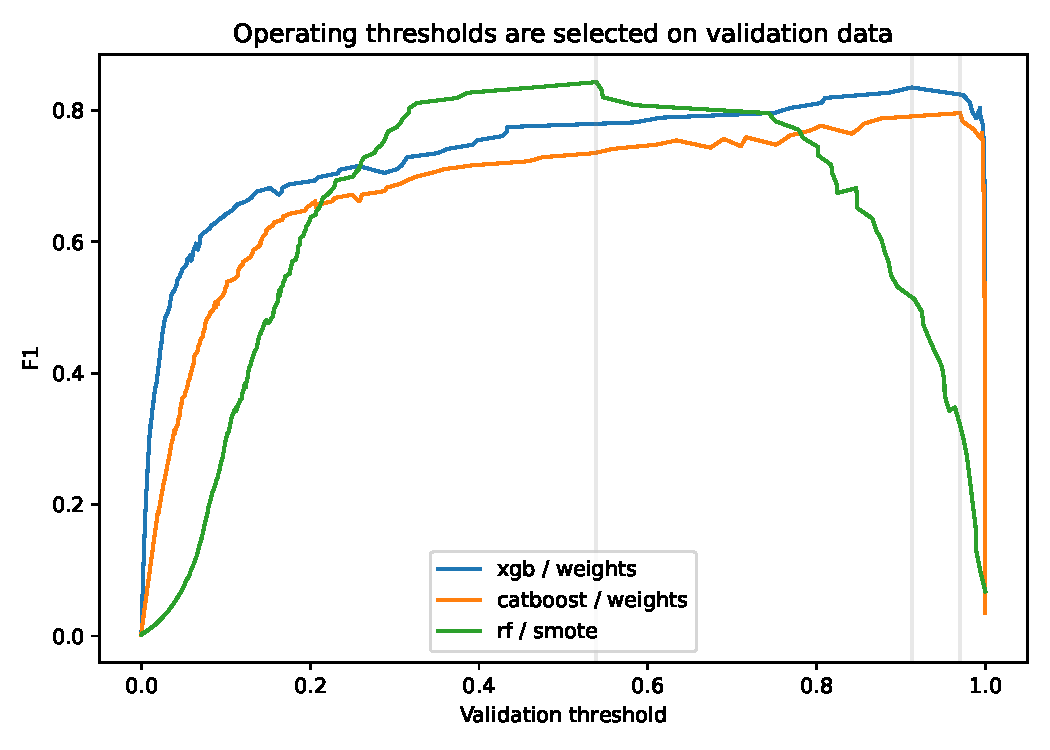
\includegraphics[width=0.95\textwidth]{figures/f10_validation_thresholds.pdf}
\caption{Validation F1 across model score thresholds. Thresholds were selected on validation data, not on the holdout; their numerical values are model-specific.}
\label{fig:thresholds}
\end{figure*}

\subsection{D. Protocol ablation}
The development-only ablation shows an A0-to-A3 mean F1 change of \RFAblationDrop{} for the forest and \XGBAblationDrop{} for XGBoost (Table~\ref{tab:ablation}). The stage means and seed spread are reported in the generated table and Fig.~\ref{fig:ablation}. A0 is legacy-like but is not an exact reproduction of the old report's fixed-threshold evaluation: it uses the deduplicated development data and selects a threshold on its own evaluation partition. A3 also uses development data only and is not comparable to the locked holdout table.

Fig.~\ref{fig:ablation} displays the bundled protocol stages over the development seeds. The larger XGBoost change cannot be assigned to scaling leakage, threshold selection, or chronology individually because the stages change several elements together.
\begin{table}[!t]
\centering
\caption{Protocol-specific development ablation across the saved seeds; stages bundle multiple changes.}
\label{tab:ablation}
\begin{tabular}{llrrrr}
\toprule Model & Protocol & F1 mean & F1 SD & PR-AUC mean & Recall mean \\
\midrule
rf & A0 legacy-like & 0.871 & 0.019 & 0.853 & 0.821 \\
rf & A1 fold-local & 0.861 & 0.026 & 0.852 & 0.825 \\
rf & A2 validation threshold & 0.857 & 0.032 & 0.838 & 0.796 \\
rf & A3 chronological & 0.823 & 0.006 & 0.744 & 0.744 \\
xgb & A0 legacy-like & 0.863 & 0.013 & 0.842 & 0.825 \\
xgb & A1 fold-local & 0.751 & 0.006 & 0.843 & 0.858 \\
xgb & A2 validation threshold & 0.841 & 0.026 & 0.835 & 0.800 \\
xgb & A3 chronological & 0.602 & 0.042 & 0.724 & 0.756 \\
\bottomrule
\end{tabular}

\end{table}
\begin{figure*}[!t]
\centering
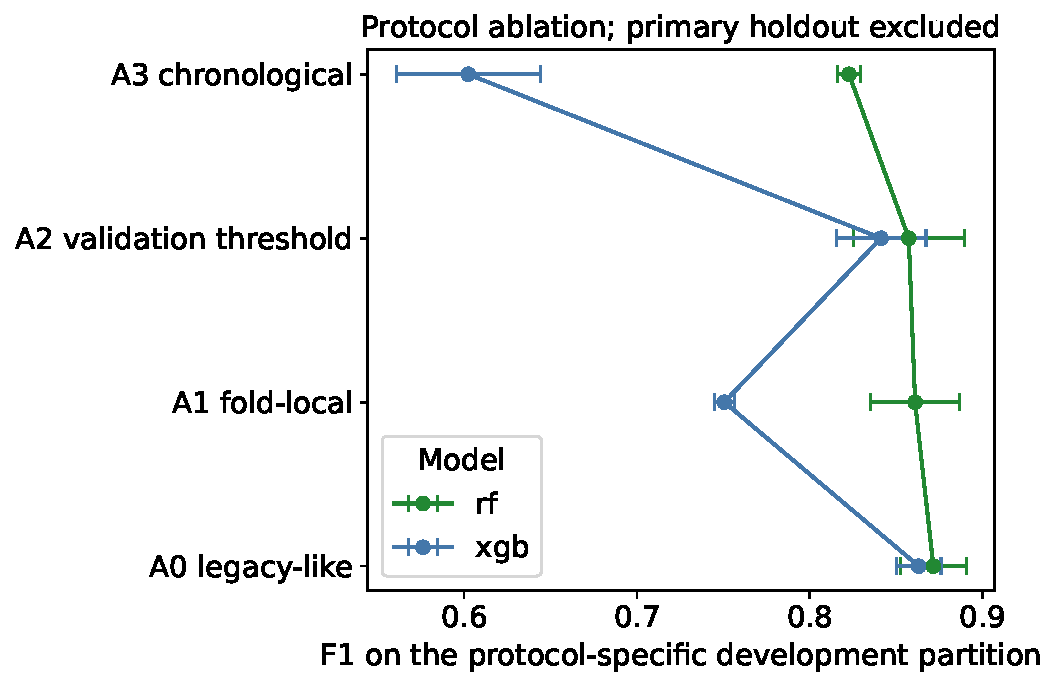
\includegraphics[width=0.95\textwidth]{figures/f12_protocol_ablation.pdf}
\caption{Development-only ablation of the legacy-like random protocol, fold-local scaling, validation thresholding, and chronological evaluation. Error bars show seed spread; the primary holdout is excluded.}
\label{fig:ablation}
\end{figure*}

\subsection{E. Explainability and error analysis}
The attribution rankings are descriptive and partly agree across methods: \SHAPPermTopTenOverlap{} features occur in both top-ten SHAP and top-ten permutation rankings, while \SHAPEDATopTenCliffOverlap{} SHAP top features occur in the top EDA effect-size ranking (Table~\ref{tab:importance}). SHAP summarizes feature contributions to predictions \cite{lundberg2017}. Table~\ref{tab:error-profile} reports the validation false-negative and true-positive counts and their median amount and hour; Fig.~\ref{fig:explainability} visualizes the attributions and case counts. These rankings describe model behavior, not causes, and the PCA components have no direct business meaning.

The validation false negatives have median amount \FNMedianAmount{} and median elapsed hour \FNMedianHour{}; true positives have median amount \TPMedianAmount{} and median elapsed hour \TPMedianHour{} (Table~\ref{tab:error-profile}). The saved validation profile contains no per-case prediction scores, so score distributions for false negatives versus true positives are unavailable without rerunning a model; no such rerun was performed.

\begin{table*}[!t]
\centering
\caption{Top attribution features and their train-only EDA ranks. The feature set shown is the union of the top SHAP and top permutation features.}
\label{tab:importance}
\begin{tabular}{lrrrr}
\toprule
Feature & Mean $|$SHAP$|$ & Permutation & $|$Cliff$|$ rank & MI rank \\
\midrule
V4 & 1.440 & 0.057 & 3 & 7 \\
V14 & 1.017 & 0.139 & 1 & 2 \\
V12 & 0.624 & 0.022 & 2 & 3 \\
hour\_sin & 0.515 & 0.000 & 22 & 15 \\
V10 & 0.351 & 0.017 & 6 & 4 \\
V11 & 0.343 & 0.006 & 5 & 5 \\
V8 & 0.300 & 0.003 & 19 & 20 \\
log1p\_amount & 0.267 & 0.001 & 25 & 22 \\
V19 & 0.232 & 0.002 & 18 & 23 \\
V7 & 0.219 & 0.006 & 9 & 10 \\
V1 & 0.187 & 0.006 & 12 & 18 \\
V3 & 0.129 & 0.004 & 4 & 8 \\
V17 & 0.181 & 0.004 & 11 & 1 \\
\bottomrule
\end{tabular}

\end{table*}
\begin{table}[!t]
\centering
\caption{Validation fraud error profile at the selected threshold.}
\label{tab:error-profile}
\begin{tabular}{lrrr}
\toprule
Validation group & Count & Median amount & Median hour \\
\midrule
False negatives & 18 & 23.735 & 12.000 \\
True positives & 39 & 45.510 & 13.000 \\
\bottomrule
\end{tabular}

\end{table}

Fig.~\ref{fig:explainability} shows which features drive the selected model's scores and how many validation fraud cases were missed or caught. The visualization cannot attach semantic or operational meaning to anonymized PCA coordinates, and the error counts are not a substitute for case-level score analysis.
\begin{figure*}[!t]
\centering
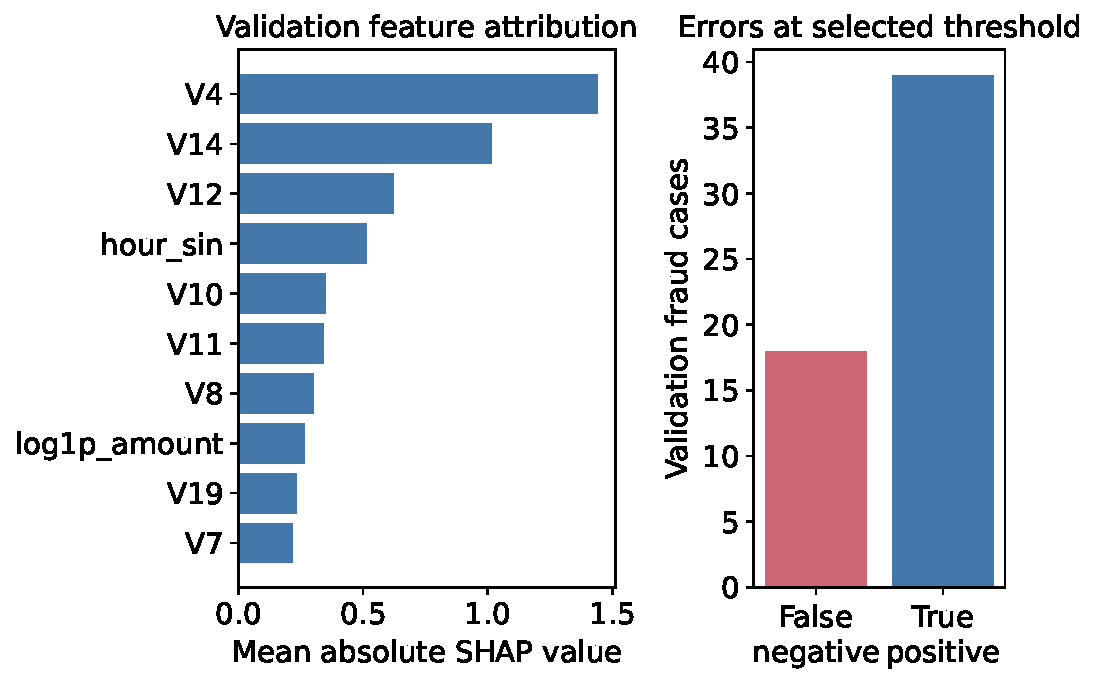
\includegraphics[width=0.95\textwidth]{figures/f14_explainability_errors.pdf}
\caption{Validation explainability and errors. Attribution ranks are descriptive; bars count false negatives and true positives at the validation-selected threshold.}
\label{fig:explainability}
\end{figure*}

\subsection{F. Calibration, cost sensitivity, and tuning}
For the saved out-of-fold logistic-regression calibration curves, the mean absolute bin gap is \CalibrationWeightsMeanAbsBinGap{} with class weights and \CalibrationSMOTEMeanAbsBinGap{} with SMOTE. This descriptive summary does not show worse calibration under SMOTE in this comparison and does not establish that resampling has no probability-shift effect for other models. The cost analysis varies review cost from \ReviewCostMin{} to \ReviewCostMax{} dataset amount units per alert; its flagged amount minus review expense is illustrative rather than measured recovery or profit (Fig.~\ref{fig:calibration-cost}). The underlying cost curve evaluates its saved scoring rule and should not be read as a deployment threshold recommendation.

The bounded tuning results are in Table~\ref{tab:tuning}. Tuned CV AP is \XgbTunedCVAP{} for XGBoost and \CatboostTunedCVAP{} for CatBoost, below their corresponding default CV means; validation AP is \XgbTunedValidationAP{} and \CatboostTunedValidationAP{}, respectively. This bounded search did not improve the saved CV comparison and did not replace the previously locked holdout choice; tuned configurations were not evaluated on the test partition.

Fig.~\ref{fig:calibration-cost} places the out-of-fold reliability curves beside the illustrative sensitivity curve. The calibration curves show similar average bin gaps, while the cost curve changes linearly with an assumed review expense and cannot establish real-world net savings.
\begin{table}[!t]
\centering
\caption{Bounded training-CV tuning and validation-only recheck.}
\label{tab:tuning}
\begin{tabular}{lrrl}
\toprule Model & Tuned CV AP & Validation AP & Parameters \\
\midrule
xgb / weights & 0.8661 & 0.7721 & min\_child\_weight=1, max\_depth=3, learning\_rate=0.05 \\
catboost / weights & 0.8652 & 0.7556 & l2\_leaf\_reg=5, depth=8 \\
\bottomrule
\end{tabular}

\end{table}
\begin{figure*}[!t]
\centering
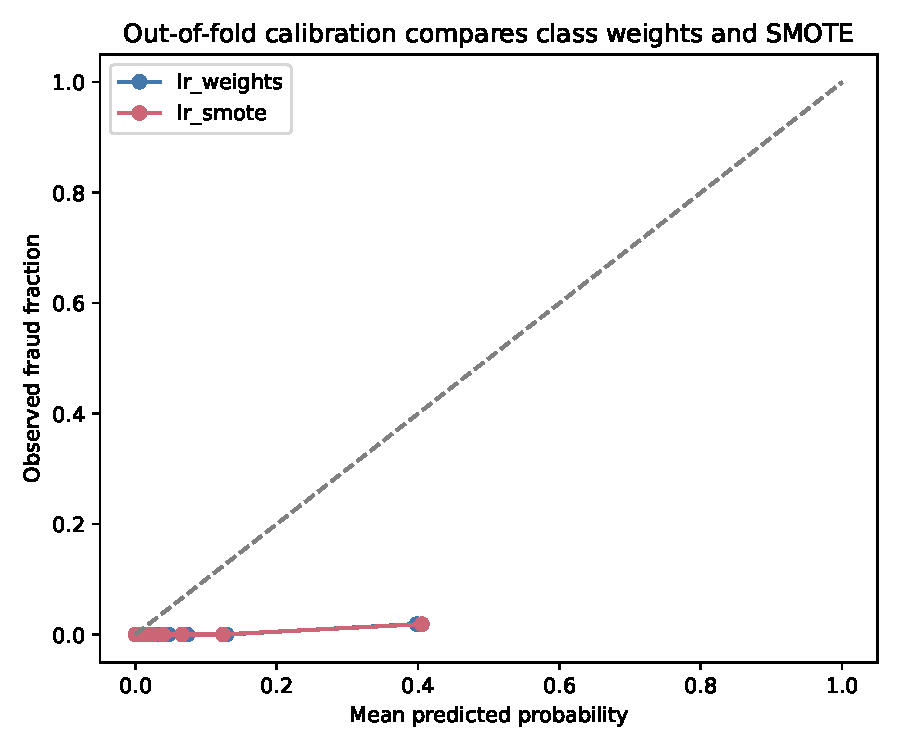
\includegraphics[width=0.48\textwidth]{figures/f11_reliability.pdf}\hfill
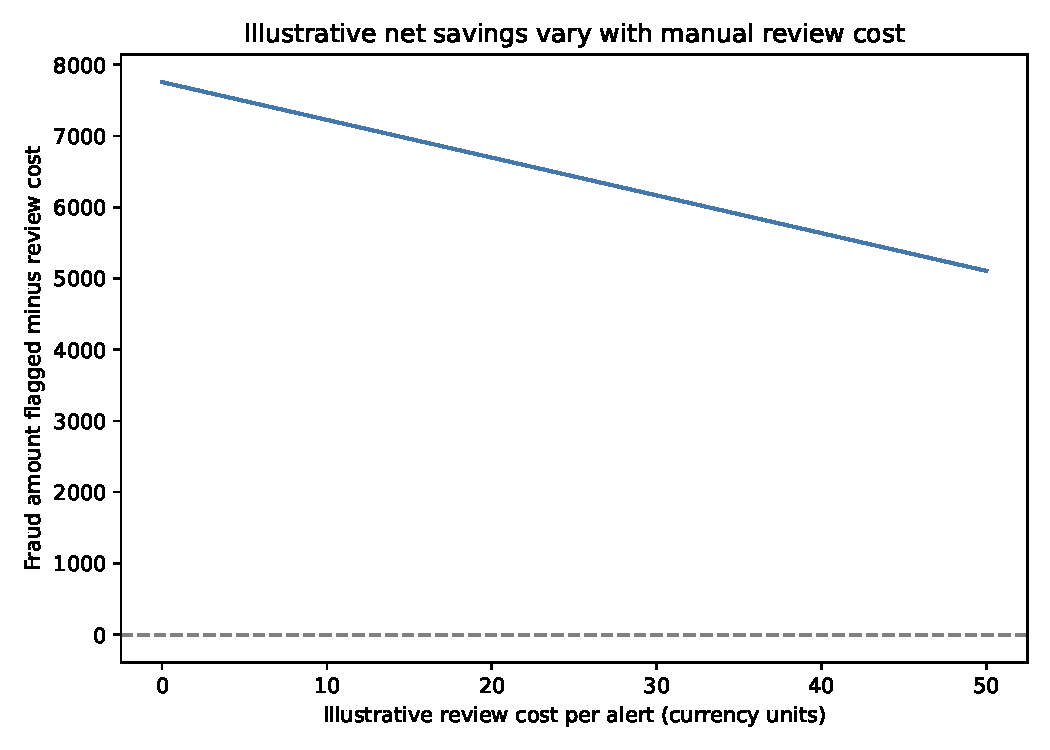
\includegraphics[width=0.48\textwidth]{figures/f13_cost_sensitivity.pdf}
\caption{Calibration and cost sensitivity. (a) Out-of-fold reliability curves compare logistic regression with class weights and SMOTE. (b) Flagged amount minus assumed review expense is an illustrative sensitivity analysis, not measured savings.}
\label{fig:calibration-cost}
\end{figure*}

\subsection{G. Hypothesis scorecard}
Table~\ref{tab:hypotheses} consolidates the pre-registered expectations and their saved outcomes. Several expectations are inconclusive or refuted, which narrows the claims supported by the study rather than invalidating the comparison. In particular, the KNN weakness and undersampling competitiveness expectations are not supported by the saved CV results.
\begin{table*}[!t]
\centering
\caption{Hypothesis outcomes transcribed from the pre-run hypothesis log and its recorded evidence.}
\label{tab:hypotheses}
\begin{tabular}{p{0.13\textwidth}p{0.22\textwidth}p{0.49\textwidth}p{0.12\textwidth}}
\toprule
Model/strategy & Hypothesis & Observed evidence & Verdict \\
\midrule
Dummy prior & PR-AUC equals prevalence and anchors no-skill performance. & CONFIRMED: test dummy PR-AUC 0.0013, matching test prevalence (74/56,746). & CONFIRMED \\
Logistic Regression + class weights & Competitive ROC-AUC, weaker PR-AUC than the strongest tree model. & INCONCLUSIVE for ROC-AUC; PR-AUC is weaker (CV 0.7107 vs XGBoost/weights 0.8717). & INCONCLUSIVE \\
Random Forest + class weights & Strong precision at moderate recall, with coarse probabilities. & INCONCLUSIVE: RF/weights was not selected for the holdout, so its operating point was not evaluated there. RF/SMOTE test precision was 0.9016 at recall 0.7432. & INCONCLUSIVE \\
KNN, k=25 + distance weights & Weakest due to 30-dimensional distance geometry and sparse minority neighbors. & REFUTED as “weakest”: KNN/no-resampling CV PR-AUC was 0.8239, above both LR strategies and all undersampling variants, though below the strongest trees. & REFUTED \\
XGBoost + class weights & Highest or near-highest PR-AUC among tested pairs. & CONFIRMED: highest CV mean PR-AUC (0.8717); holdout PR-AUC 0.7952. & CONFIRMED \\
CatBoost + class weights & On par with XGBoost and stable across folds. & INCONCLUSIVE: CV mean 0.8676 with SD 0.0497; the paired top-two holdout PR-AUC difference CI includes zero, so there is no evidence of a difference. & INCONCLUSIVE \\
SMOTE strategies & Ranking and threshold behavior may shift; resampling occurs inside each training fold. & PARTLY CONFIRMED: fold-local SMOTE scored well for RF (CV PR-AUC 0.8667) but the strategy-level mean (0.826) was similar to weights (0.827). Threshold effects are model-specific. & PARTLY CONFIRMED \\
Undersampling strategies & Ranking may remain useful while posterior probabilities shift. & REFUTED as a competitive ranking hypothesis here: strategy-level mean CV PR-AUC was 0.688, below weights (0.827) and SMOTE (0.826). Calibration/prior shift is addressed separately in S7. & REFUTED \\
\bottomrule
\end{tabular}

\end{table*}
\FloatBarrier

\section{Discussion}
\label{sec:discussion}
The main findings are as follows. First, train-only cross-validation selects XGBoost with class weights, but the leading candidates are close relative to fold variability and the top-CV-pair holdout interval contains zero. Second, the forest with SMOTE has the largest observed holdout AP, yet its paired comparison with the CV-selected XGBoost candidate does not provide clear evidence of a difference; selection should therefore remain tied to the predeclared CV rule. Third, undersampling has lower CV AP than weights or SMOTE for the tree models, while logistic regression slightly favors SMOTE over weights. Fourth, the A0-to-A3 changes are larger for XGBoost than the forest, but they are bundled development contrasts rather than causal measurements of leakage.

These estimates are more conservative than a protocol that allows evaluation data to affect scaling, threshold choice, or model selection because the chronological holdout remains outside those choices. The ablation is consistent with protocol-dependent performance changes, but it cannot quantify the isolated optimism caused by any one fault. The old report's values are not used as findings or copied as results.

The internal validity is limited by the single chronological holdout, its \TestFraudCount{} fraud cases, and threshold selection from \ValidationFraudCount{} validation fraud cases; threshold metrics can change when only a few cases move between decisions. External validity is limited to one anonymized dataset spanning \TimeSpanHours{} hours, without card or merchant identifiers and without a long-term drift test. Construct validity is limited because AP summarizes ranking rather than review workload or recovered value, and the review-cost curve uses illustrative assumptions rather than observed review outcomes.

Three departures from the initial plan affect interpretation. The hyperparameter search was bounded to a small number of settings per top CV model rather than the maximum planned search size, so tuning is exploratory. A0 is legacy-like and does not reproduce the old fixed-threshold benchmark exactly. Finally, model selection uses stratified shuffled folds inside the chronological training partition rather than time-ordered CV folds; the final validation and test partitions remain chronological, but within-training fold estimates do not simulate forward-only deployment.
\FloatBarrier

\section{Conclusion}
\label{sec:conclusion}
Under the leakage-controlled selection protocol, XGBoost with class weights is the primary candidate at mean CV AP \PrimaryCVAP{}, but its holdout AP of \XgbWeightsAP{} is not clearly separated from the forest's \RfSmoteAP{} because their paired interval includes zero (Tables~\ref{tab:cv} and~\ref{tab:holdout-ranking}; Fig.~\ref{fig:holdout}). The development ablation changes mean F1 by \RFAblationDrop{} for the forest and \XGBAblationDrop{} for XGBoost from A0 to A3, but the bundled stages do not identify how much change is caused by leakage alone (Table~\ref{tab:ablation}; Fig.~\ref{fig:ablation}). Deployment conclusions require evaluation beyond this \TestFraudCount{}-fraud holdout and \TimeSpanHours{}-hour window, including delayed labels, longer temporal coverage, and measured review outcomes that this study does not contain (Table~\ref{tab:splits}; Fig.~\ref{fig:calibration-cost}).
\FloatBarrier

\section{Future Work}
\label{sec:future}
Future studies should evaluate additional chronological windows and explicitly simulate delayed fraud verification. They should measure how alert budgets, investigator capacity, and confirmed recovery affect an operating policy. Where governance permits, card or merchant context could be added to test whether the anonymized feature conclusions generalize. Prospective monitoring should measure calibration and ranking changes over time rather than assume stability from a short benchmark.
\FloatBarrier

\appendices
\section{Saved model settings and fit times}
\label{app:settings}
Table~\ref{tab:hyperparameters} lists the selected per-model settings from the saved configuration snapshot, with the evaluated imbalance strategy for each CV row. The fit-time column in Table~\ref{tab:cv} reports the mean training time per fold; it is not an end-to-end runtime estimate.
\begin{table*}[!t]
\centering
\caption{Saved model settings for each evaluated model-strategy pair.}
\label{tab:hyperparameters}
\begin{tabular}{llp{0.54\textwidth}}
\toprule
Model & Strategy & Saved model settings \\
\midrule
catboost & SMOTE & iterations=500, depth=6, learning\_rate=0.05, task\_type=CPU \\
catboost & undersampling & iterations=500, depth=6, learning\_rate=0.05, task\_type=CPU \\
catboost & class weights & iterations=500, depth=6, learning\_rate=0.05, task\_type=CPU \\
knn & none & n\_neighbors=25, weights=distance \\
knn & undersampling & n\_neighbors=25, weights=distance \\
lr & SMOTE & C=1, max\_iter=2000 \\
lr & undersampling & C=1, max\_iter=2000 \\
lr & class weights & C=1, max\_iter=2000 \\
rf & SMOTE & n\_estimators=300, min\_samples\_leaf=2 \\
rf & undersampling & n\_estimators=300, min\_samples\_leaf=2 \\
rf & class weights & n\_estimators=300, min\_samples\_leaf=2 \\
xgb & SMOTE & n\_estimators=300, learning\_rate=0.05, max\_depth=6, tree\_method=hist \\
xgb & undersampling & n\_estimators=300, learning\_rate=0.05, max\_depth=6, tree\_method=hist \\
xgb & class weights & n\_estimators=300, learning\_rate=0.05, max\_depth=6, tree\_method=hist \\
\bottomrule
\end{tabular}

\end{table*}
\FloatBarrier

\bibliographystyle{IEEEtran}
\bibliography{references}
\end{document}
